% !TeX spellcheck = en_GB
% !TeX program = lualatex
%
% v 2.3  Feb 2019   Volker RW Schaa
%		# changes in the collaboration therefore updated file "jacow-collaboration.tex"
%		# all References with DOIs have their period/full stop before the DOI (after pp. or year)
%		# in the author/affiliation block all ZIP codes in square brackets removed as it was not %         understood as optional parameter and ZIP codes had bin put in brackets
%       # References to the current IPAC are changed to "IPAC'19, Melbourne, Australia"
%       # font for ‘url’ style changed to ‘newtxtt’ as it is easier to distinguish "O" and "0"
%
\documentclass
[
    a4paper,
    %boxit,        % check whether paper is inside correct margins
    %titlepage,    % separate title page
    %refpage       % separate references
    biblatex,     % biblatex is used
    %keeplastbox,   % flushend option: not to un-indent last line in References
    %nospread,     % flushend option: do not fill with whitespace to balance columns
    %hyphens,      % allow \url to hyphenate at "-" (hyphens)
    %xetex,        % use XeLaTeX to process the file
    %luatex,       % use LuaLaTeX to process the file
]{jacow}
%
% ONLY FOR \footnote in table/tabular
%
\usepackage{pdfpages,multirow,ragged2e} %

%
% To define glossaries
%
\usepackage[acronym]{glossaries}

%
% if BibLaTeX is used
%
\ifboolexpr{bool{jacowbiblatex}}%
 {%
  \addbibresource{references.bib}
 }{}
\listfiles

%
% New commands
%
\newcommand*{\rom}[1]{\uppercase\expandafter{\romannumeral#1\relax}}
\providecommand{\der}{\mathrm{d}}
\providecommand{\rf}{\mathrm{rf}}
\providecommand{\wrf}{\omega_\rf}
\providecommand{\frf}{f_\rf}
\providecommand{\Real}[1]{\ensuremath{\mathrm{Re}\left\{#1\right\}}}

%
% Glossaries
%
\newacronym{3hc}{3HC}{third-harmonic cavity}
\newacronym{dcct}{DCCT}{direct-current current transformer}
\newacronym{dft}{DFT}{discrete Fourier transform}
\newglossaryentry{bbb}
{
    name={BbB},
    description={bunch-by-bunch feedback system},
    first={bunch-by-bunch (\glsentrytext{bbb}) feedback system},
}
\newglossaryentry{hom}
{
    name={HOM},
    description={higher-order mode},
    first={\glsentrydesc{hom} (\glsentrytext{hom})},
    plural={HOMs},
    descriptionplural={higher-order modes},
    firstplural={\glsentryplural{hom}}
}


\begin{document}
\title{Broadband impedance induced heating proxy for operation at higher total current at SIRIUS}
\author
{
    F. H. de Sá\thanks{murilo.alves@lnls.br}\textsuperscript{1},
    I. C. de Almeida\textsuperscript{1},
    M. B. Alves\textsuperscript{1,2},
    G. Gomes\textsuperscript{3},
    L. Lin\textsuperscript{1},
    X. Resende\textsuperscript{1}\\
    \textsuperscript{1}Brazilian Synchrotron Light Laboratory--LNLS, Campinas, Brazil\\
    \textsuperscript{2}Gleb Wataghin Institute of Physics, University of Campinas--UNICAMP, Campinas, Brazil\\
    \textsuperscript{3}Brazilian Center for Research in Energy and Materials--CNPEM, Campinas, Brazil
}
\maketitle

\begin{abstract}
    SIRIUS is a 4\textsuperscript{th} generation synchrotron light source built and operated by the Brazilian Synchrotron Light Laboratory (LNLS), in Campinas, Brazil. Currently, SIRIUS storage ring operates in top-up mode at 100 mA in uniform fill. The main limiting factor for reaching higher currents is the temporary RF system in use. It is comprised of one PETRA 7-Cell cavity and two solid state amplifier towers that combined provide at most 120kW of power. By mid 2024, two superconducting RF cavities will replace the current cavity and two amplifier towers will be added to the system, allowing operation at higher currents. The design current of SIRIUS storage ring is 350 mA, which can only be achieved once a third harmonic cavity is installed to lengthen the bunches to avoid excessive wake-induced heating of sensitive components. However, the installation of such cavity is not foreseen in the near future, which raises the question of which is the maximum current in uniform fill SIRIUS can be operated. This work will present some theoretical and experimental studies carried out to answer this question.
\end{abstract} 

\section{Introduction}
    SIRIUS RF power plant upgrade will be ready for commissioning in October of 2024. Once this system is operating, it will allow increasing the stored current in users operations to~\SI{350}{\milli\ampere} with the design nominal voltage of~\SI{3}{\mega\volt}, considering the energy loss by dipoles and all the undulators of Phase~\rom{1} of operation. The expected natural bunch length at this voltage is approximately~\SI{2.4}{\milli\meter}. This short bunch imposes a large wake-field induced heat-load on the accelerator components and shorten the Touschek Lifetime of the machine. A~\gls{3hc} is considered to lengthen the bunches and alleviate these effects, but its installation is not planned for the near future. For this reason, it is important to estimate the maximum stored current SIRIUS storage ring can operate without the~\gls{3hc}.

    One way to estimate the heating load for higher currents involves using different filling patterns. Most of the heating load of SIRIUS storage ring is due to broadband impedances, according to the model. For this type of wake-field the heat-load depends on the squared sum of the filling pattern and on the total current squared. This fact is useful for SIRIUS because the current total power available by the RF system limits the maximum stored current to~\SI{100}{\milli\ampere}, with a gap voltage of~\SI{\sim1.57}{\mega\volt}. SIRIUS operates with uniform filling, which has the smallest possible squared sum. In this way, by using any other filling patterns at~\SI{100}{\milli\ampere}, we can estimate the heating load of the uniform filling at higher currents.

    Another way of estimating the heat-load consists in decreasing the gap voltage of the cavity. The power consumption of the cavity itself decreases, which allows increasing the total stored current. Currently, SIRIUS operates with a PETRA 7-Cell cavity at a gap voltage of~\SI{\sim1.57}{\mega\volt} with a total power of~\SI{\sim100}{\kilo\watt}. From this,~\SI{\sim50}{\kilo\watt} is used to keep the gap voltage and the remaining power is consumed by the~\SI{100}{\milli\ampere} beam. Decreasing the gap voltage to~\SI{\sim0.7}{\mega\volt} would still keep Touschek lifetime above~\SI{1}{\hour} (the energy loss per turn in SIRIUS storage ring is~\SI{\sim480}{\kilo\electronvolt}) and allow the maximum stored current to increase to~\SI{\sim170}{\milli\ampere}. This method has the advantage of keeping the same filling pattern of regular operation, thus sampling the impedance at the same harmonics, which also serves as an estimate of the effect of narrow band impedance sources. On the other hand, the bunch length is larger at lower gap voltages, which limits the frequency range of the impedance sampled by the beam and underestimate the broadband effect. 

    This work will describe the experimental and theoretical studies carried out estimate the maximum beam current SIRIUS can operate, while keeping a reasonable lifetime for top-up operation and no heating issues.

\section{Theory of Heating Load}
    The power deposited by the beam in a component of the vacuum chamber is given by
    \begin{equation}\label{eq:power_general}
        P = I_\mathrm{t}^2T_0 \frac{\omega_0}{2\pi}\sum_{p=-\infty}^{\infty} \left|\tilde{\lambda}(p\omega_0)\right|^2\Real{Z(p\omega_0)},
    \end{equation}
    where $I_\mathrm{t}>0$ is the total current of the beam, $T_0$ and $\omega_0$ are the revolution period and angular frequency of the storage ring, $Z$ is the longitudinal impedance of the component and 
    \begin{equation}
        \tilde{\lambda}(\omega) = \int_{-\infty}^\infty\der z \lambda(z) e^{i\omega z/c},
    \end{equation}
    where $c$ is the speed of light and $\lambda(z)$ is the longitudinal distribution of the beam, which can be written as
    $
        \lambda(z) = \sum_{\ell=0}^{h-1} F_\ell \lambda_\ell(z - \ell \lambda_\rf)
    $,
    where $h$ is the harmonic number of the ring, $\lambda_\rf=cT_0/h$ is the rf wavelength, $\lambda_\ell(z)$ is the distribution of the $\ell$-th bunch and $F_\ell \ge 0$ are the components of the filling pattern vector,
    $
    F = \left(\frac{I_0}{I_\mathrm{t}},\dots, \frac{I_{h-1}}{I_\mathrm{t}}\right)^\mathrm{T}
    $,
    which sums to unity. Since the bunch distributions are normalized to unity, then the beam distribution is also normalized to unity.
    
    The Fourier transform of the longitudinal distribution is then given by
    $
        \tilde{\lambda}(\omega) = \sum_{\ell=0}^{h-1}F_\ell\tilde{\lambda_\ell}(\omega)e^{i\ell\omega \lambda_\rf/c}
    $
    and its squared modulus is
    \begin{equation}\label{eq:modulus_squared}
        \left|\tilde{\lambda}(\omega)\right|^2 = \left|\tilde{\lambda_0}(\omega)\right|^2 \left|B(\omega)\right|^2,
    \end{equation}
    where we defined the quantity $B(\omega) = \sum_{\ell=0}^{h-1}F_\ell e^{i\ell\omega \lambda_\rf/c}$
    and assumed all bunch distributions are equal to $\lambda_0(z)$.

    Inserting Eq.~\eqref{eq:modulus_squared} in Eq.~\eqref{eq:power_general}, we get
    \begin{equation}
        P = I_\mathrm{t}^2T_0 \frac{\omega_0}{2\pi}\sum_{p=-\infty}^{\infty} \left|\tilde{\lambda_0}(\omega_p)\right|^2 \left|B(\omega_p)\right|^2\Real{Z(\omega_p)},
    \end{equation}
    where $\omega_p = p\omega_0$. Note that
    $
        B(p\omega_0) = \sum_{\ell=0}^{h-1}F_\ell e^{i2\pi p\ell} = \mathrm{DFT}(F)^*_p,
    $
    where $\mathrm{DFT}(F)^*_p$ denotes the complex conjugate of the $p$-th component of the \gls{dft} of the filling pattern vector. Since the filling pattern has length $h$, its \gls{dft} has the property:
    $
        B((p+h)\omega_0) = B(p\omega_0)
    $,
    which allows us to write the power loss in the following convenient form
    \begin{equation}
        P = I_\mathrm{t}^2T_0 \frac{\omega_0}{2\pi}\sum_{\ell=0}^{h-1} \left|B(\ell\omega_0)\right|^2\sum_{p=-\infty}^{\infty} \left|\tilde{\lambda_0}(\omega_{p,l})\right|^2 \Real{Z(\omega_{p,l})},
    \end{equation}
    where $\omega_{p,l} = (ph+\ell)\omega_0$.
    
    Now, if we assume the impedance varies slowly in the frequency scale of the rf frequency, i.e., it is a broad band impedance,
    $
        Z((ph+\ell)\omega_0) \approx Z(ph\omega_0), \, \forall\, p \in\mathbb{Z}\,\,\mathrm{and}\,\, \ell \in[0,h-1],
    $
    and remembering the Parseval's theorem for the~\gls{dft}~\cite{Wikipedia_DFT},
    $
        \sum_{\ell=0}^{h-1} \left|B(\ell\omega_0)\right|^2 = h\sum_{\ell=0}^{h-1} F_\ell^2 = h|F|^2,
    $
    we can write the power loss as
    \begin{equation}
        P \approx I_\mathrm{t}^2 \left|F\right|^2 T_0 \frac{h\omega_0}{2\pi}\sum_{p=-\infty}^{\infty} \left|\tilde{\lambda_0}(\bar{\omega}_p)\right|^2 \Real{Z(\bar{\omega}_p)},
    \end{equation}
    where $\bar{\omega}_p = ph\omega_0$. Defining the loss factor
    $
        \kappa = \frac{h\omega_0}{2\pi}\sum_{p=-\infty}^{\infty} \left|\tilde{\lambda_0}(\bar{\omega}_p)\right|^2 \Real{Z(\bar{\omega}_p)}
    $,
    the power loss can be summarized as
    \begin{equation}\label{eq:power_broadband}
        P \approx I_\mathrm{t}^2 \left|F\right|^2 T_0\, \kappa.
    \end{equation}
    Note it depends on the square of the total current stored and on the modulus squared of the filling pattern vector, which is minimum for uniform filling, $|F|^2=1/h$, and maximum for a single-bunch, $|F|^2=1$. Also, for simplified filling patterns with $M$ arbitrarily spaced bunches with the same current per bunch, we have $|F|^2=1/M$.

\section{Model Calculations}

    Figure~\ref{fig:model_vary_vgap}
    \begin{figure}
        \centering
        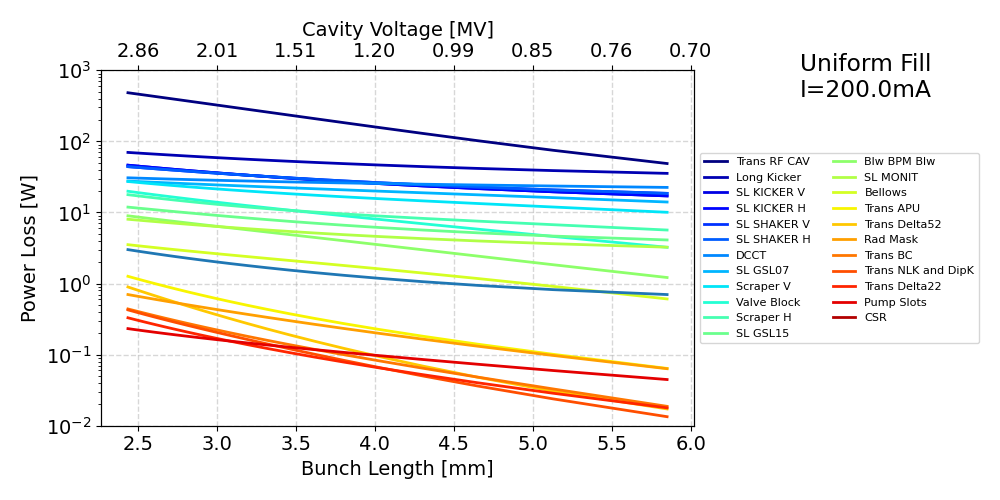
\includegraphics[width=0.48\textwidth]{vary_vgap_uniform_fill_curr200p00mA.png}
        \caption{Power loss for each component of the impedance budget model as function of the cavity voltage and bunch length.}
        \label{fig:model_vary_vgap}
    \end{figure}
     shows the power loss predicted by the impedance budget model of the SIRIUS storage ring for each component of the vacuum chamber when the gap voltage of the cavity is varied and uniform filling is considered. Note the strong dependence of the power loss with the bunch length. Figure~\ref{fig:model_vary_fillp}
    \begin{figure}
        \centering
        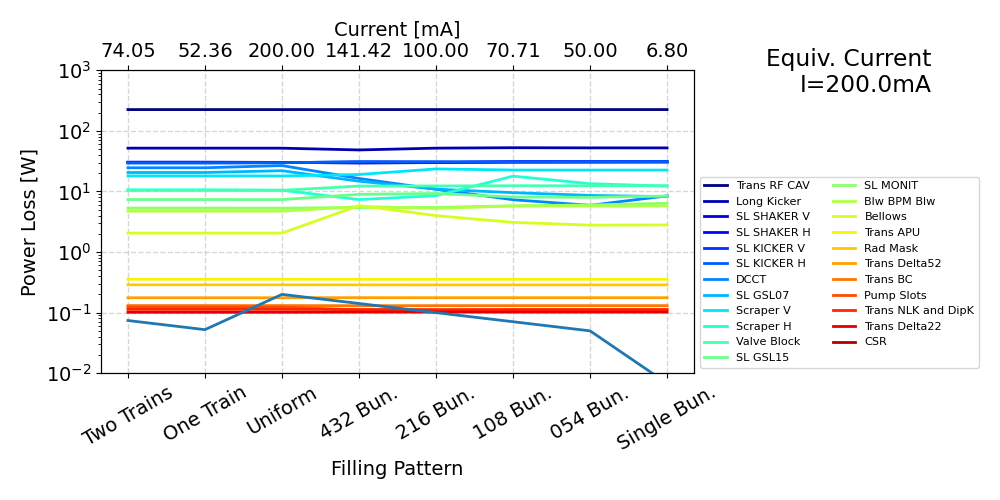
\includegraphics[width=0.48\textwidth]{vary_fillp_equivcurr200p00mA.png}
        \caption{Power loss for each component of the impedance budget model for several filling patterns. The total current used for each filling pattern was calculated using Eq.~\eqref{eq:power_broadband} so that the equivalent current in uniform filling was kept constant and equal to~\SI{200}{\milli\ampere}. The nomenclature~"$\!N$ Bun." refers to fillings with~$N$ equally spaced bunches.}
        \label{fig:model_vary_fillp}
    \end{figure}
     shows the model prediction for power loss for different filling patterns, keeping the equivalent total power constant, according to Eq.~\eqref{eq:power_broadband}. Since most components are dominated by broad band impedances, the power loss do not depend too much on the filling pattern.
    
    From these results we see that the taper transition of the superconducting rf cavities is the single component with the larger power loss reaching approximately~\SI{225}{\watt} at~\SI{200}{\milli\ampere} in uniform filling and~\SI{1.6}{\mega\volt} in the rf cavities. Since this component is not installed yet, it will not be possible to check future heating problems. However, this power load was considered in thermal simulations of this component. The second class of components with large power deposition are the striplines, ranging from~\SIrange{20}{50}{\watt} of deposited power.

\section{Experimental results}

    Two machine studies were conducted to probe both approaches of estimation of heat-load. The method of decreasing the cavity voltage was tested first. In practice, the lower cavity voltage reduced the synchrotron tune, decreasing the longitudinal coupled-bunch instability threshold induced by the cavity \glspl{hom}. With the lower tune, the instability was stronger than what is controllable by the~\gls{bbb}. We started with a low gap voltage of~\SI{\sim0.9}{\mega\volt} and increased the current from zero. At~\SI{64}{\milli\ampere} the beam instability started to compromise the low level RF control and we had to increase the voltage. We followed this strategy along the rest of the experiment and reached~\SI{150}{\milli\ampere} with a gap voltage of~\SI{1.35}{\mega\volt} and using~\SI{120}{\kilo\watt} of power. During this study no temperature increase was noted in any sector of the storage ring.
    
    The study with non-uniform fillings started with a single train of filled buckets, as shown in Fig.~\ref{fig:2023-08-01_onetrain_fill}.
    \begin{figure}
        \centering
        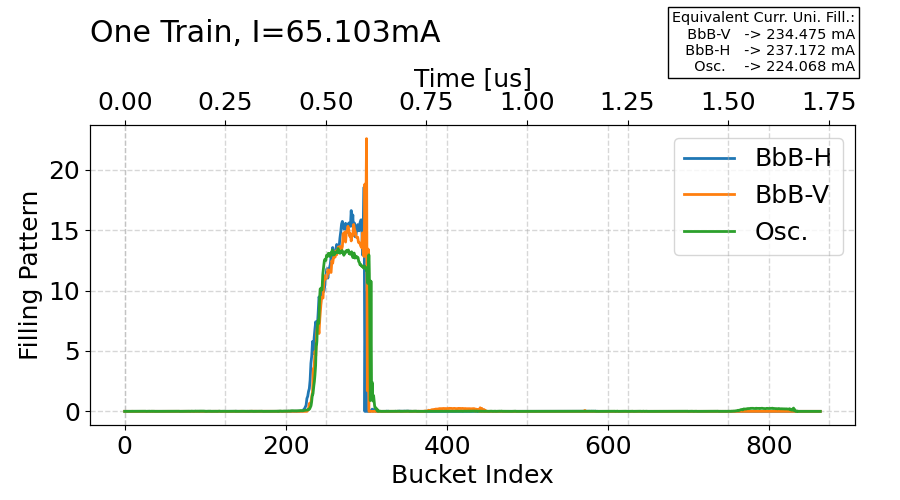
\includegraphics[width=0.48\textwidth]{trains1_run3_curr65p103.png}
        \caption{Filling pattern estimation by three different systems. The text shows the equivalent current calculated using each filling.}
        \label{fig:2023-08-01_onetrain_fill}
    \end{figure}
    In this run,~\SI{65}{\milli\ampere} was reached with a single train in the machine. The current could not be increased any further because the temperature of the cavity window was too close from its interlock threshold of~\SI{100}{\celsius}. This high temperature was being induced by coupled-bunch oscillations of the beam, due to \glspl{hom} of the cavity. The current was kept constant in top-up mode for some time to analyse the evolution of the pressure and temperature of the components. No pressure related problems were observed, but some temperature from sector~\num{1} increased significantly and did not stabilize during the whole experiment, reaching~\SI{\approx53}{\celsius} before the beam was dumped, see Fig.~\ref{fig:temps_sector1}.
        \begin{figure}
        \centering
        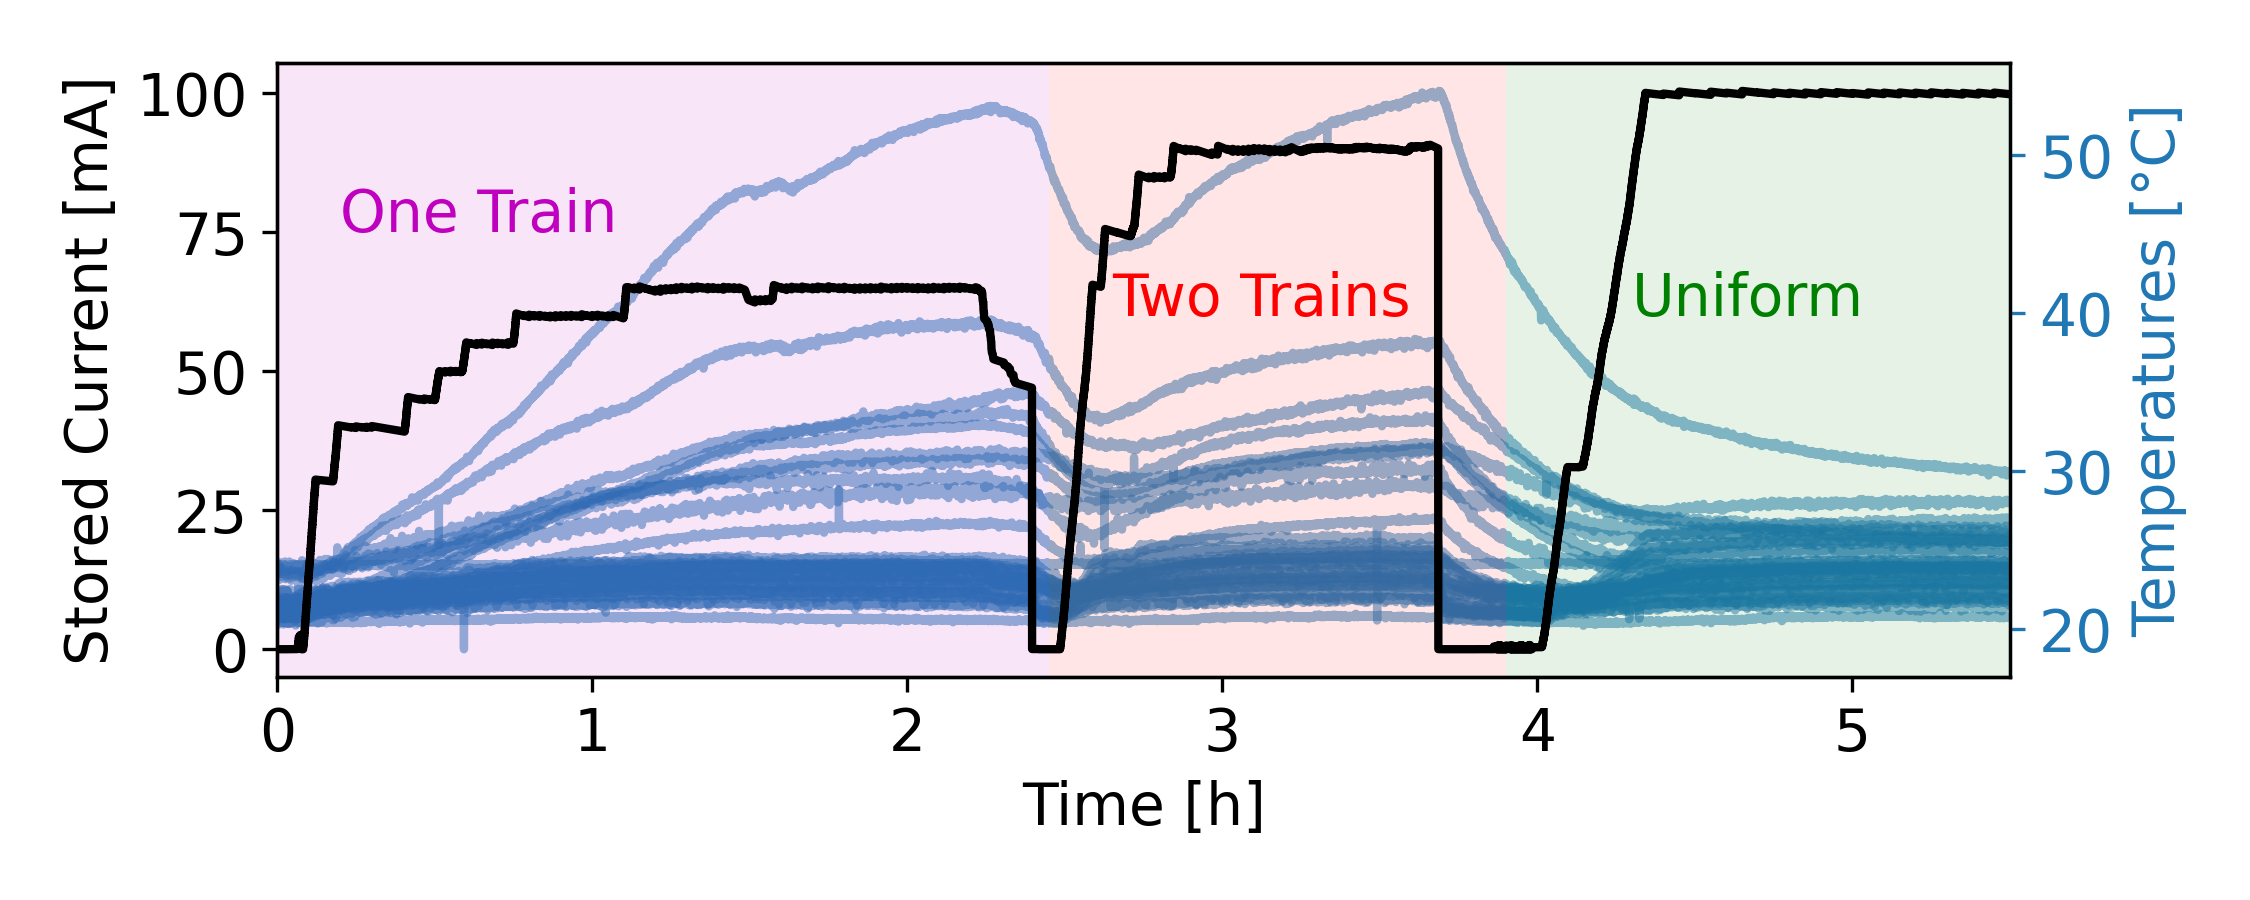
\includegraphics[width=0.5\textwidth]{temps_sector1.png}
        \caption{Filling pattern estimation by three different systems. The text shows the equivalent current calculated using each filling.}
        \label{fig:temps_sector1}
    \end{figure}
    % Unfortunately, it was not possible to identify which component was the source of the observed heating.

    Next, the beam was injected in two trains. Figure~\ref{fig:2023-08-01_twotrains_fill}
    \begin{figure}
        \centering
        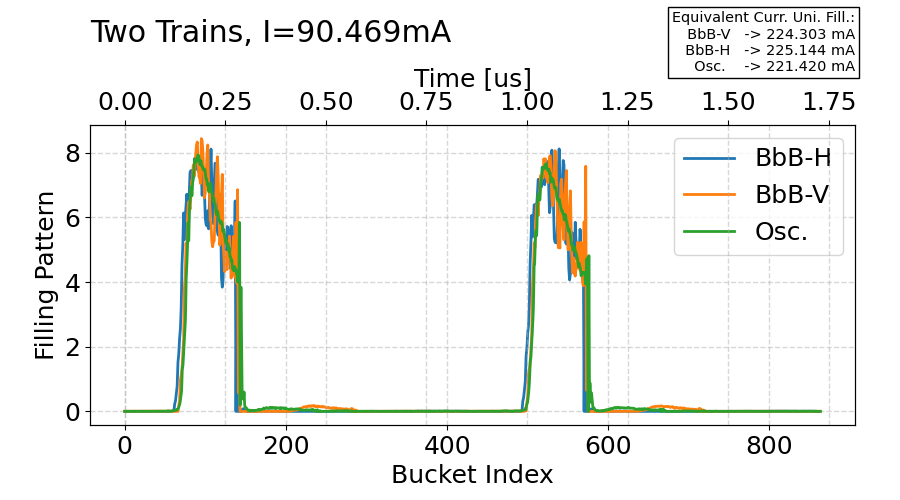
\includegraphics[width=0.48\textwidth]{trains2_run1_curr90p469.png}
        \caption{Filling pattern estimation by three different systems. The text shows the equivalent current calculated using each filling.}
        \label{fig:2023-08-01_twotrains_fill}
    \end{figure}
    shows the equivalent current of this filling pattern. In this configuration, it was possible to reach~\SI{90}{\milli\ampere}, keeping he temperature of the cavity window at~\SI{96}{\celsius}. The same heating problem was observed in sector 1. Figure~\ref{fig:temps_sector1} shows the similarity between the heating of the single train experiment with the one with two trains. Both experiments had similar equivalent currents, as shown in Figs~\ref{fig:2023-08-01_onetrain_fill} and~\ref{fig:2023-08-01_twotrains_fill}. This observation corroborates with the hypothesis of broadband induced power on the component close to the sensor.

\section{Conclusion}

This study aimed to access the heating load of operations at higher currents with different proxies. The method based on different filling patterns has shown to be more efficient for such verification in the case of SIRIUS, because it conserves the bunch length. In this context, it was shown experimentally that SIRIUS will probably be able to operate at~\SI{200}{\milli\ampere} without the need of the~\gls{3hc}. 
%
% only for "biblatex"
%
\ifboolexpr{bool{jacowbiblatex}}%
	{\printbibliography}%
	{%
	% "biblatex" is not used, go the "manual" way
	
	%\begin{thebibliography}{99}   % Use for  10-99  references
	\begin{thebibliography}{9} % Use for 1-9 references

   \bibitem{Lima:IPAC22-TUPOST014}
   A. P. B. Lima, I. Carvalho de Almeida, D. Daminelli, R. H. A. Farias, M. Hoffmann Wallner, and F. K. G. Hoshino,
   \textquotedblleft{Sirius Storage Ring RF System Status Update}\textquotedblright,
   in \emph{Proc. IPAC’22}, Bangkok, Thailand, Jun. 2022, pp. 872--875.
   \url{doi:10.18429/JACoW-IPAC2022-TUPOST014}

    \bibitem{Venturini2018}
    M. Venturini,
    ``Passive higher-harmonic rf cavities with general settings and multibunch instabilities in electron storage rings,''
    \emph{Phys. Rev. Accel. Beams 21} 114404 (2018)

    \bibitem{He2022b}
    T. He,
    \textquotedblleft Novel perturbation method for judging the stability of the equilibrium solution in the presence of passive harmonic cavities \textquotedblright in
    \emph{Phys. Rev. Accel. Beams} \textbf{25}, 094402 (2022)

    \bibitem{He2022a}
    T. He, W. Li, Z. Bai, and L. Wang,
    \textquotedblleft Periodic transient beam loading effect with passive harmonic cavities in electron storage rings\textquotedblright~in \emph{Phys. Rev. Accel. Beams} \textbf{25}, 024401 (2022)
    
    \bibitem{Cullinan2024}
    F. J. Cullinan, \AA{}. Andersson, J. Breunlin, M. Brosi, and P. F. Tavares,
    \textquotedblleft Experimental observation of a mode-1 instability driven by Landau cavities in a storage ring \textquotedblright in \emph{Phys. Rev. Accel. Beams 27}, 044403 (2024)

    \bibitem{CollectiveEffectsRepo}
    F. H. de Sá and M. B. Alves,
    ``pycolleff and cppcolleff: Modules for impedance analysis and wake-field induced instabilities evaluation'' (2023),
    \url{https://doi.org/10.5281/zenodo.8088076}

    \bibitem{Suzuki1983}
    T.~Suzuki, Y.~Chin, and K.~Satoh,
    \textquotedblleft Mode Coupling Theory and Bunch Lengthening in {SPEAR} {II} \textquotedblright
    \emph{Part. Accel.} \textbf{13} (1983), 179-198,
    KEK Preprint 82-26

    \bibitem{AlvesSa2023}
    M. B. Alves and F. H. de S\'a,
    ``Equilibrium of longitudinal bunch distributions in electron storage rings with arbitrary impedance sources and generic filling patterns,''
    \emph{Phys. Rev. Accel. Beams 26}, 094402 (2023)

    \bibitem{Lindberg2018}
    R. R. Lindberg,
    ``Theory of coupled-bunch longitudinal instabilities in a storage ring for arbitrary rf potentials,''
    \emph{Phys. Rev. Accel. Beams 21}, 124402 (2018)
	\end{thebibliography}
} % end \ifboolexpr


\end{document}

